\documentclass[12pt,a4paper]{article}
\usepackage[]{color}
\usepackage[]{graphicx}
\usepackage[utf8x]{inputenc}
\usepackage{amsfonts}
\usepackage{amsmath}
\usepackage{amssymb}
\usepackage{eepic}
\usepackage{epic}
\usepackage{fullpage}
\usepackage{listings}
\usepackage{parskip}
\usepackage{ucs}
\usepackage{verbatim}
\usepackage{pgfplots}
\usepackage{xcolor}

\title{
    {\normalsize\sc ID1217 Concurrent Programming} \\ 
    {\large Programming Project} \\
    Parallelize Particle Simulation
}

\author{
    \bf Saurav Puri \\
    \bf  sauravpuri200@gmail.com\\
}

\lstset{%
basicstyle=\small,  % print whole listings small
}

\begin{document}

\maketitle

\section{Objective}
The main objective of this project is to develop parallel applications in shared and distributed memory models and practice improving the performance of parallel applications. The task is to parallelize a particle simulator that shows the interaction of numerous forces on a select particle. The particles are only affected by the neighboring particles within a certain range. The density of the particles is set sufficiently low so that given $n$ particles, only $O(n)$ interactions are expected. The algorithm is given; however, the implementation runs in $O(n\textsuperscript{2})$. The goal of this project is to create a sequential program that runs in $T = O(n)$ and parallel programs using Pthreads, OpenMP, and MPI that run in $T/p$ when using $p$ processors. 

\section{Environment}
This project was made on Mac iOS using XCode and ran on Scientific Linux 6.7 Carbon using a remote server connection to home university. The runtime values were collected around similar time, to minimize remote machine error.

\section{Approach}
My approach to this task was to first, understand the provided code and understand the algorithm used to perform the task in $O(n\textsuperscript{2})$ time. I began with the serial implementation because serial would be the most basic task to tackle. The serial algorithm checks every particle for interaction with the selected particle. Due to the small density, only the neighboring particles have an impact. So this is where time can be saved.

I used an ADT to index through all the particles to find which particles would have a force on the current particle selected.

\subsection{ADT}

The ADT class holds references to all the particles. The structure creates a grid and one particle is put into each cell. The ADT class has an insert function that implements this. The grid can now be divided into larger neighborhoods. Within these neighborhoods, the relevant particles would have an effect on each other. Now, it becomes easy to determine which particles are close enough to have a force on the current particle. The indexing through neighboring particles can be done in $O(n)$ time for every particle because: 
\begin{itemize}
  \item Indexing is constant
  \item The backend vector class $push\textunderscore back$ function is constant
  \item There are finite interactions on every particle
\end{itemize}
Therefore, iterating over all the particles in the ADT can be done in $O(n)$ time. 

For all of the algorithms, I inserted all the particles into the grid and then distributed the particles to different threads/processes.

\subsection{Shared Memory Implementation - Pthreads}

The Pthread implementation of the algorithm required a barrier to synchronize the multiple threads. The same barrier could be reused multiple times. By using a barrier, the program is segmented into three portions
\begin{itemize}
  \item forces are calculated for the particle interactions,
  \item then, the particles are moved,
   \item finally, the particles are stored to their new position on the ADT by the main thread, thread 0.
\end{itemize}

\subsection{Shared Memory Implementation - OpenMP}

The OpenMP implementation of the algorithm required the main thread to create and allocate work to other threads. Each of the portions mentioned above requires its own $for$ loop and the corresponding parallelization. There is no need to add a manual barrier in OpenMP because after each $for$ loop is parallelized, there is a implicit barrier. 

\subsection{Distributed Memory Implementation -  MPI}

The MPI implementation had one key design choice. I chose to implement the parallelization to resemble a shared memory model. By doing this, the design matches very closely to the other 2 parallel implementations. The main process initializes all the particles and broadcasts this on a shared "bus." Each process then takes these particle locations and inserts it onto its own grid. Then the process calculates the forces on its own particles based on the neighbors, as done in the other two implementations. Then the process broadcasts its own new updated location and gathers information about all the other particles from the other processes from the same shared "bus."

\section{Analysis with Graphs}

The Figures below shows the runtime of the serial, Pthread, OpenMP, MPI implementations. The plots show that the implementation runs in $O(n)$. 

\fcolorbox{black}{blue}{\rule{0pt}{6pt}\rule{6pt}{0pt}}\quad Serial

\fcolorbox{black}{red}{\rule{0pt}{6pt}\rule{6pt}{0pt}}\quad Pthreads

\fcolorbox{black}{green}{\rule{0pt}{6pt}\rule{6pt}{0pt}}\quad OpenMP

\fcolorbox{black}{black}{\rule{0pt}{6pt}\rule{6pt}{0pt}}\quad MPI


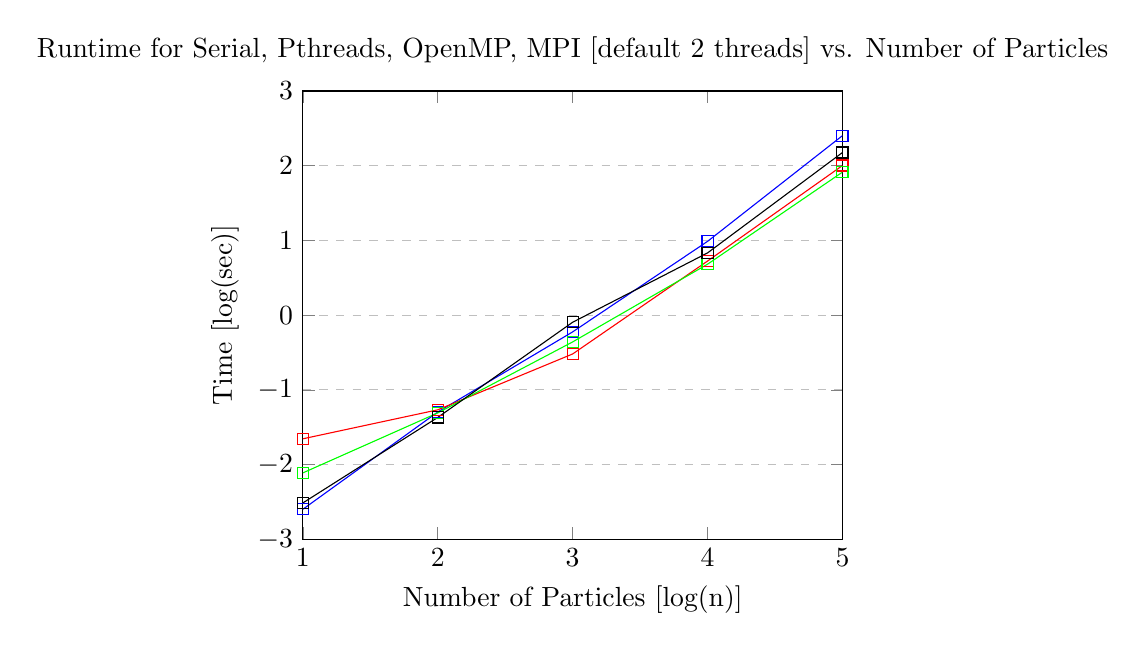
\begin{tikzpicture}
\begin{axis}[
    title={Runtime for Serial, Pthreads, OpenMP, MPI [default 2 threads] vs. Number of Particles},
    xlabel={Number of Particles [log(n)] },
    ylabel={Time [log(sec)]},
    xmin=1, xmax=5,
    ymin=-3, ymax=3,
    xtick={1 ,2 , 3, 4, 5},
    ytick={-3 ,-2,-1 , 0, 1, 2, 3},
    legend pos=north west,
    ymajorgrids=true,
    grid style=dashed,
]
 
\addplot[
    color=blue,
    mark=square,
    ]
    coordinates {
    (1, -2.5989)(2, -1.2974)(3, -.2245)(4, .987)(5, 2.402)
    };
\addplot[
    color=red,
    mark=square,
    ]
    coordinates {
    (1, -1.65569)(2, -1.2677)(3, -0.5200)(4, .723378)(5,2.002)
    };
    \addplot[
    color=green,
    mark=square,
    ]
    coordinates {
    (1, -2.112)(2, -1.3091)(3, -.3588)(4, .6813)(5, 1.91394)
    };
\addplot[
    color=black,
    mark=square,
    ]
    coordinates {
    (1, -2.514)(2, -1.3695)(3, -.09541)(4, .8325)(5, 2.176)
    };
 
\end{axis}
\end{tikzpicture}



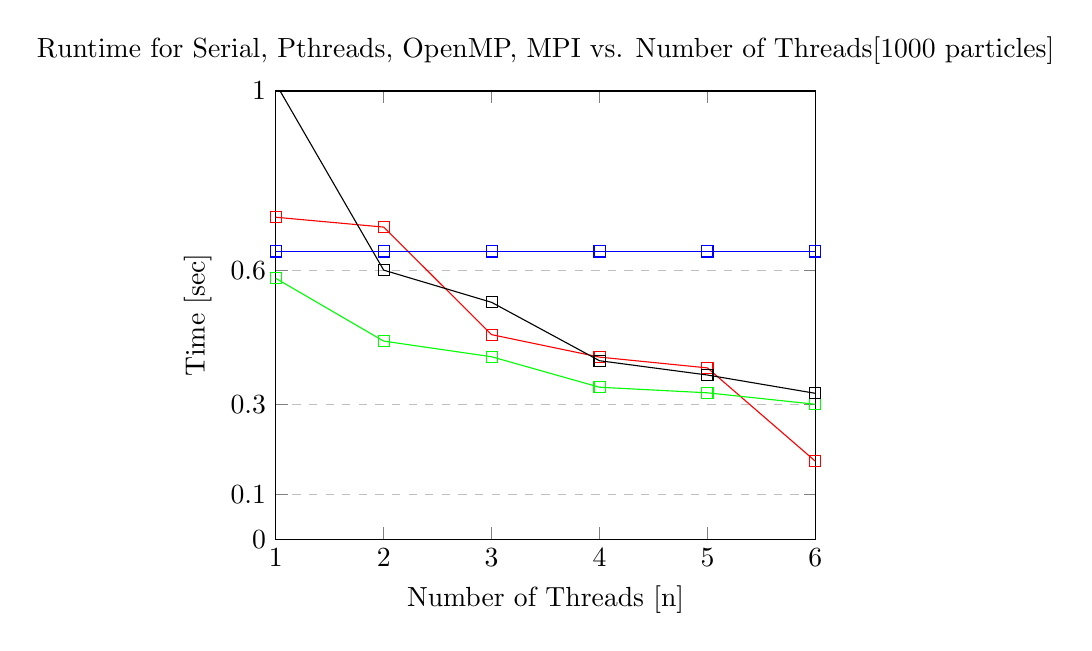
\begin{tikzpicture}
\begin{axis}[
    title={Runtime for Serial, Pthreads, OpenMP, MPI vs. Number of Threads[1000 particles]},
    xlabel={Number of Threads [n] },
    ylabel={Time [sec]},
    xmin = 1, xmax = 6,
    ymin= 0, ymax = 1,
    xtick={1, 2, 3, 4, 5, 6},
    ytick={0, .1, .3, .6 , 1},
    legend pos=north west,
    ymajorgrids=true,
    grid style=dashed,
]
 
\addplot[
    color=red,
    mark=square,
    ]
    coordinates {
    (1, 0.718317)(2, 0.696345)(3, 0.456412)(4, 0.406301)(5, 0.382242)(6, 0.174056)
    };
        \addplot[
    color=green,
    mark=square,
    ]
    coordinates {
    (1, 0.582025)(2, 0.442043)(3, 0.407116)(4, 0.339111)(5, 0.326679)(6, 0.301161)
    };
\addplot[
    color=black,
    mark=square,
    ]
    coordinates {
(1, 1.01671)(2, 0.600363)(3, 0.528496)(4, 0.398267)(5, 0.366356)(6, 0.325512)
    };
    \addplot[
    color=blue,
    mark=square,
    ]
    coordinates {
(1, 0.642025)(2, 0.642025)(3, 0.642025)(4, 0.642025)(5, 0.642025)(6, 0.642025)
    };


\end{axis}
\end{tikzpicture}


By analyzing the graphs, it is clear the algorithms run in $O(n)$ and it is also evident that performance of the parallel algorithms could be better. The initialization overhead for OpenMP and MPI surpass the serial speed, while Pthreads does not have too much overhead but the speedup increases much more slowly. 


\section{Conclusion}

As seen by the graphs in the previous section, the parallelized code does not reach the idealized T/$p$ runtime. The main reason for the lower speedup would be optimizations in the code and additional added overhead when trying to parallelize the algorithm. 

In the shared memory model implementation, the insertion of particles onto the ADT is done serially, because, this was the most obvious solution to change the $O(n\textsuperscript{2})$ runtime to $O(n)$. However, the insertions could have been done in parallel using concepts similar to matrix multiplication, where each thread takes a column or row. By parallelizing the insertion, the algorithm would require another synchronization point, so that no thread begins processing forces before all the points have been inserted to the grid. But, this synchronization not be as slow as serially entering each particle one by one. 

The distributed memory implementation is non-resourceful when implementing the communication background. In my implementation, every particle is sent to every process, which is definitely not necessary. This will definitely increase the runtime, but would still be able to run bounded by $O(n)$. A better method would be to calculate which particles are needed per process; but that would require a significant amount of calculations and error checking, and could also be costly. This is very similar to the matrix multiplication concept in ideals, but in practice very different to implement.  

The ADT implementation succeeds in running the algorithms in $O(n)$ time and works fine to reduce the runtime from $O(n\textsuperscript{2})$. However, the ADT structure may not be the best idea to achieve ideal parallelism of the algorithm. This is because, creating the ADT structure will always take $O(n)$. Data structures like AVL trees and Binary Search trees can insert values in $O(log(n))$ and search for values in $O(log(n))$. 

From this project I learned the importance of viewing algorithms in a whole different manor when implementing it in parallel. I also learned that the best way to achieve maximum parallelism is by choosing the correct data structure through analysis and trial-error.  


\appendix


\end{document}
